\label{chap:3}

\section{Relação Tempo-Frequência}
    
    \subsection{Contexto}
        Para o caso real, os sinais de áudio convoluem com a resposta ao impulso de um filtro, que representa o percurso percorrido pelos mesmos das fontes aos sensores. Isto caracteriza um caso de misturas convolutivas (conforme visto na Seção \ref{sec:separability}). 
        
        Com o conhecimento de que podemos implementar a operação de convolução de sinais no domínio tempo pela  multiplicação no domínio da frequência, uma forma de simplificar este problema seria aplicar a transformada de Fourier a estes sinais, resolver a separação de misturas instântaneas e aplicar a transformada inversa de Fourier para levar os sinais de volta ao domínio do tempo. Uma das vantagens desta abordagem reside na redução da complexidade computacional, estando algoritimo ICA que trabalhe com números complexos e misturas instantâneas apto para ser usado.
        
        Entretanto, as ambiguidades de escalamento e permutação inerentes ao problema de BSS (Seção \ref{sec:separability}) tornam elementos centrais no processo de separação e precisam ser resolvidas. Ao trabalhar no domínio da frequência, a ICA fornece componentes independentes em cada raia de frequência, mas as componentes de cada fonte devem ser corretamente agrupadas antes de serem levadas para o domínio do tempo. Isto é crucial para obter uma solução aceitável.
        
        Também é relevante citar o problema da circularidade da DFT. No caso mais geral de sinais e sistemas discretos, o produto no domínio da frequência corresponde à convolução circular no domínio do tempo. Isto restringe o uso dessa propriedade ao caso em que os filtros no domínio do tempo são periódicos, o que não é condizente com a realidade. Para fazer com que na nossa aplicação a multiplicação no domínio da frequência seja equivalente à convolução linear no domínio do tempo, é necessário que o de raias de frequência (tamanho da DFT) seja maior ou igual ao tamanho do filtro somado ao trecho do sinal que está sendo processado, além do sinal ter de ser reconstruído através da técnica de \textit{Overlap-Add} \cite{signalprocessing} . Este processo é conhecido como \textit{FFT Filtering} e é amplamente utilizada para realizar convolução rápida de um filtro de ordem elevada com um sinal longo. Quando esta condição no tamanho da DFT não é respeitada, o sinal provinente do tratamento no domínio da frequência, seguido da sua IDFT será uma versão distorcida do sinal equivalente à convolução no domínio do tempo.
        
        Outro ponto fundamental sobre trabalhar no domínio da frequência é que introduzimos um caráter complexo aos sinais do nosso sistema devido às transformadas necessárias para a mudança de domínio. Conforme citado na Seção \ref{sec:ICA}, embora vários algoritmos ICA tenham sido desenvolvidos para trabalhar com sinais reais, eles podem ser estendidos para o caso complexo, desde que tenha sido apropriadamente escolhida a função $G$ (maximização da não-gaussianidade) ou a função \textit{score} (estimação da ML). 
        
    \subsection{Sumário}
        O processo de tratamento do problema de FDBSS, ilustrado na Figura \ref{fig:frequencymodel}, pode ser estruturado da seguinte forma:
        
        \begin{enumerate}
            \item Inicialmente, transformam-se os vetores de misturas $\mathpzc{x_j}(n)$, $j = 1,\dots,M$ em suas representações no domínio da frequência $\mathpzc{x_j}(m,k)$, $k = 0, \dots, K-1$ (sendo $m$ o índice do \textit{frame} e $K$ o número de raias de frequência), através da \textit{STFT} (do inglês, \textit{Short Time Fourier Transform});
            
            \item Como etapa de pré-processamento, realiza-se o branqueamento dos sinais, obtendo-se os sinais $\mathpzc{z_j}(m,k)$ e a matriz branqueadora $\mathbf{V}$($\mathpzc{k}$);
            
            \item A etapa de processamento, que consiste na separação propriamente dita, é realizada gerando uma matriz separadora $\mathbf{W}$($\mathpzc{k}$) para cada raia de frequência $k$, além do vetor com as saídas separadas $\mathbf{y}$($\mathpzc{m,k})$ = [$\mathpzc{y_1}$($\mathpzc{m,k})$, $\dots$, $\mathpzc{y_N}$($\mathpzc{m,k})$]$^T$;
            
            \item Como pós-processamento, são resolvidas as questões de permutação e escalamento, através das matrizes $\mathbf{P}$($\mathpzc{k})$ e $\mathbf{\Lambda}$($\mathpzc{k})$;
            
            \item Por fim, é necessário levar o vetor com as saídas separadas para o domínio do tempo através da \textit{ISTFT} (do inglês, \textit{Inverse Short Time Fourier Transform}).
            
        \end{enumerate}

        \begin{figure}[h!]
            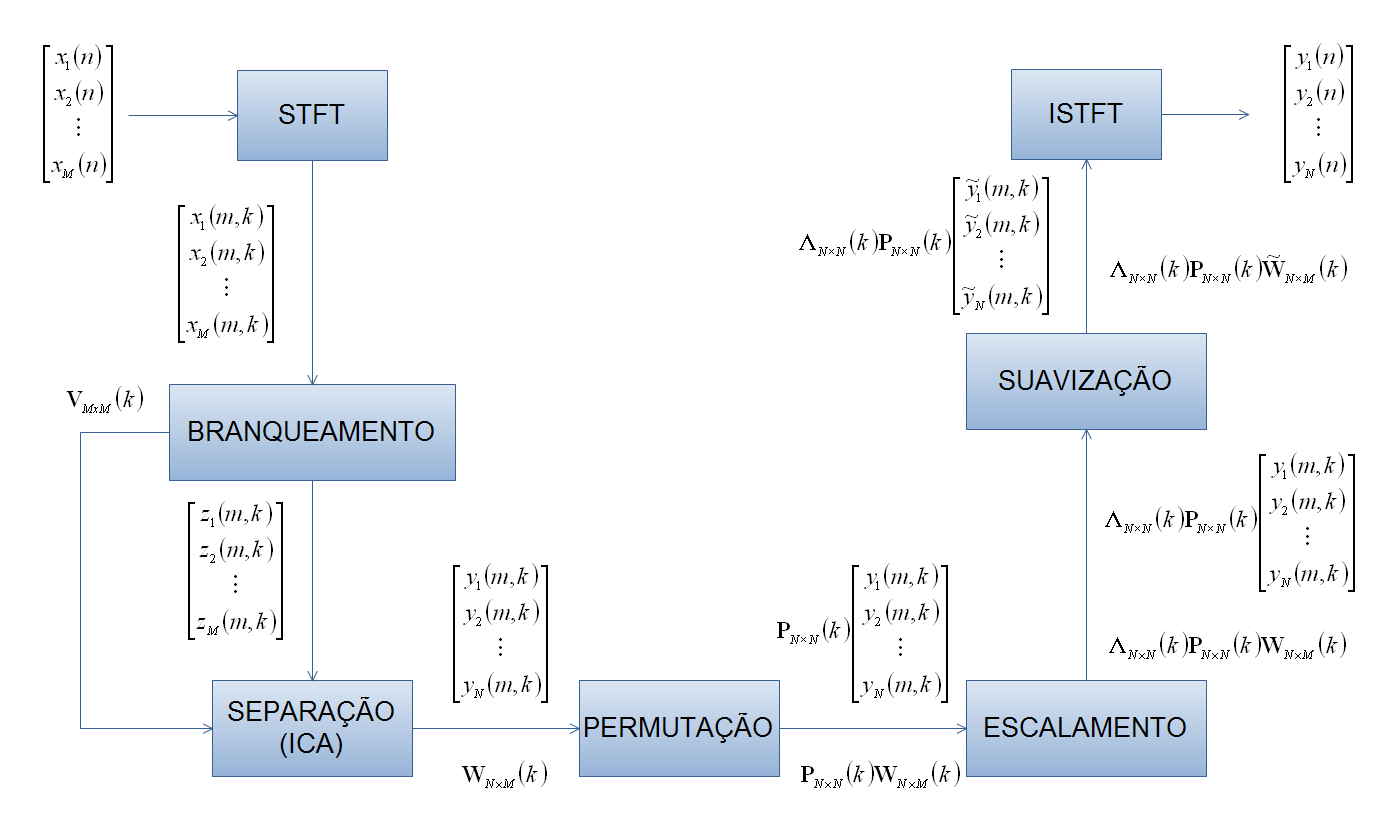
\includegraphics[scale=0.4]{frequencyprocess.png}
            \caption{Esquema do processo de FDBSS.}
            \label{fig:frequencymodel}
        \end{figure}

    \subsection{STFT} \label{sec:stft}
        A STFT de um sinal x é dada pela equação:

    %STFT
    \begin{equation}\label{eq:STFT}
        \mathbf{X}(\mathpzc{m},\mathpzc{k})
        = \sum_{n} x(\mathpzc{n})
        \mathpzc{win}_\mathpzc{a}(\mathpzc{n} - \mathpzc{mJ})
        exp \left( -j \frac{2\pi\mathpzc{kn}}{K} \right), \mathpzc{k} = 0, \dots, K-1
    \end{equation}
    onde:
    \begin{itemize}
        
        \item $k$ é a raia de frequência, com intervalo [0, $K$-1]. Pode ser interpretada como a frequência discreta $\mathpzc{f_k}$ $\in$ \big\{0,$\frac{1}{K}$ $\mathpzc{f_s}$, \dots, $\frac{K-1}{K}$ $\mathpzc{f_s}$ \big\};
                    
        \item $K$ é o número de raias de frequência da DFT;
                    
        \item $L$ é o comprimento da janela;
                    
        \item $J$ é o deslocamento da janela;
        
        \item  $\mathpzc{f_s}$ é a frequência de amostragem;
        
        \item $\mathpzc{win_a}$($\mathpzc{n}$) é a janela de análise, definida como sendo não-nula apenas no intervalo [0, L-1]. O salto J é obviamente menor ou igual L, ou haverá perda de observações. Este salto deve ser bem escolhido para não haver distorções na síntese dos sinais.
    \end{itemize}
    
        Em geral, utiliza-se $K=L$ na equação acima. Entretanto, há casos em que $K>L$, chamados de \textit{oversampled}. Nestes casos, é necessário utilizar \textit{zero-padding} para preencher o sinal com zeros antes de passar para a frequência, conforme descrito em \cite{STFT}.
        
        Uma notação prática para o cálculo da STFT é dada por:


        \begin{equation}\label{eq:practiceSTFT}
            \mathbf{X}(\mathpzc{m})
            = DFT(diag(\mathbf{x_{frame}}(\mathpzc{m})\mathbf{win_a}))
         \end{equation}
         onde 
        \begin{enumerate}
        
            \item \textit{DFT}($\mathbf{v})$ representa a DFT do vetor $\mathbf{v}$, que pode ser calculada através da FFT;
            
            \item O vetor $\mathbf{x_{frame}}$(m) = [$\mathpzc{x}$($\mathpzc{mJ}$), $\dots$, $\mathpzc{x(mJ + L - 1)}$]$^T$ tem comprimento $L$ e representa o \textit{frame m} no domínio do tempo;
            
            \item O vetor $\mathbf{X}(\mathpzc{m})$ = [${X}$($\mathpzc{f_0,m})$, $\dots$, $\mathbf{X}$(${f_{K-1},m}$)]$^T$ tem comprimento $K$ e corresponde à representação em
            frequência do \texit{frame m};
            
            \item O vetor $\mathbf{win_a}$ contém os elementos não nulos da janela mostrada na equação (\ref{eq:STFT}). Assim sendo, tem comprimento $L$. O produto diag($\mathbf{x}$($\mathpzc{mJ}$))$\mathbf{win_a}$ resulta em um vetor de comprimento $L$. Por conta disso, se $K>L$, devem ser realizado \texit{zero-padding} de $K-L$ amostras no final do vetor, antes de aplicar a DFT.
        
        \end{enumerate}
        
        Uma notação prática correspondente ao cálculo da ISTFT está é dada pelas equações:
        
        \begin{equation}\label{eq:practiceISTFT}
            \mathbf{y_{frame}}(\mathpzc{m})
            = diag(\mathbf{win_s}IDFT(\mathbf{Y}(\mathpzc{m}))
         \end{equation}
        
        \begin{equation}\label{eq:practiceISTFT2}
            \mathbf{y}(\mathpzc{n})
            = \sum_{m}\text{shift}(\mathbf{y_{frame}}(\mathpzc{m}),\mathpzc{mJ},\mathbf{N_{amost}})
         \end{equation}
        
        O sinal $\mathbf{y}$($\mathpzc{n}$) tem o comprimento de $N_{amost}$ e a operação shift($\mathbf{a}$,b,c) desloca o vetor $\mathbf{a}$ de b amostras e aumenta seu comprimento para c, de forma que o vetor resultante tem no total $P$ elementos não-nulos, onde $P$ é o tamanho do vetor $\mathbf{a}$.
        
        A técnica de \textit{Overlap-Add} consiste em acrescentar \textit{frames} superpostos para formar o sinal completo. Também conhecida como OLA, esta técnica possui algumas variações, tais como a WOLA (\textit{Weighted Overlap-Add}) e a COLA (\textit{Constant Overlap-Add}). Esta técnica utiliza-se de uma janela de síntese $\mathpzc{win_s}(n)$ para a realização da ISTFT. Relacionar a janela de síntese $\mathpzc{win_s}(n)$ com a janela de análise $\mathpzc{win_a}(n)$ é fundamental para criar condições para que a transformação de volta para o domínio do tempo não possua distorções. 
        
        Para que a \textit{FFT Filtering} gere um resultado satisfatório, as condições \ref{eq:condition1} e \ref{eq:condition2} devem ser satisfeitas. A condição \ref{eq:condition2} é chamada de COLA.
        
        \begin{equation}\label{eq:condition1}
            K \geq L + Q - 1
        \end{equation}
        
        \begin{equation}\label{eq:condition2}
            \sum_m \mathpzc{win_a(n - mJ) = c},\text{c constante}, \forall\mathpzc{n} \in \mathbb{Z}
        \end{equation}
        
        \begin{equation}\label{eq:condition3}
            \sum_m \mathpzc{win_a(n - mJ)}\mathpzc{win_s(n - mJ) = c}, \text{c constante}, \forall\mathpzc{n} \in \mathbb{Z}
        \end{equation}
        
        
        Neste trabalho, iremos utilizar a janela de \texit{Hanning}, representada em \ref{eq:hanning}, como janela de análise, atendendo à condição COLA \ref{eq:condition2}. Para isto, usaremos J = $\frac{L}{2}$. Normalmente, a janela retangular é escolhida como a janela de síntese. Existem estudos acerca da utilização de outras janelas e em quais condições estas satisfazem ou não à condição COLA. Recomendamos a leitura de \cite{LuizVictorio} para maior aprofundamento no assunto.
        
        \begin{equation}\label{eq:hanning}
            \mathpzc{w_{hanning}(n)} = 0,5 \left( 1 - cos\frac{2\pi\mathpzc{n}}{L}\right)
        \end{equation}
        
        Em suma, quando trabalhamos no domínio da frequência utilizando STFT, para cada raia de frequência $k$, buscaremos suas contribuições em todos os saltos de janela $L$ e aplicaremos o método de separação escolhido.
        
\section{Pré-Processamento}
        O estágio de pré-processamento pode ser necessário, auxiliar ou desnecessário, dependendo do método de separação a ser empregado no processamento propriamente dito. O método mais comum de pré-processamento é o do branqueamento, que se baseia na média do vetor de amostras.
    
    \subsection{Branqueamento} \label{sec:whitening}
        Em geral, branquear os vetores é uma boa prática, visto que faz grande parte do trabalho de separação, a descorrelação. Dependendo do método utilizado na etapa de separação, o branqueamento pode ser obrigatório (FastICA) ou pode melhorar a velocidade e robustez da convergência do algoritmo ICA no domínio da frequência (Natural ICA). A normalização do vetor de misturas desempenha um papel importante em sinais de áudio devido à sua característica de não-brancura (ou colorimento), ou seja, a energia varia bastante entre as suas componentes de frequências.
        
        Matematicamente, é possivel mostrar que o processo de branqueamento faz aproximadamente metade do trabalho de separação, sem muito custo computacional. Entre outros benefícios, estão a rapidez e uniformidade na convergência para cada raia de frequência, quando utilizado um passo de adaptação fixo, além de ser pré-requisito dos algoritmos FastICA.
        
        O processo é dividido em duas partes. A primeira consiste em fazer a centralização do vetor de misturas, isto é, fazer com que cada mistura possua média igual a zero. Feito isso, é necessário tornar a sua matriz de covariância igual à matriz identidade, resultando na descorrelação das componentes do vetor de amostras.
        
        A centralização pode ser realizada individualmente sobre cada uma das raias de frequência do vetor de amostras no domínio da frequência $\mathpzc{x_{jk}}(m)$, de forma a obter $\mathpzc{x_{jk}}(m)$ $\leftarrow$ $\mathpzc{x_{jk}}(m)$ - $\mathpzc{E}$$\{$$\mathpzc{x_{jk}(m)}$$\}$.
        
        Uma vez feita a centralização, tem-se que $\mathpzc{E}$$\{$$\mathbf{x}$$\}$ = 0 . Assim sendo, a matriz de covariância do vetor de misturas é dada por:
        
        \begin{equation}\label{eq:covariance}
            \mathbf{R_x} = \mathpzc{E}\{\mathbf{xx^T}\}
        \end{equation}
        
        O branqueamento se dá sobre cada frequência por uma matriz \mathbf{V}:
        
        \begin{equation}\label{eq:whiteningfrequency}
            \mathbf{z} = \mathbf{V}\mathbf{x}
        \end{equation}
        
        Para obtermos o vetor $\mathbf{z}$ com as suas componentes descorrelacionadas, precisamos encontrar a matriz branqueadora $\mathbf{V}$ tal que $\mathpf{R_z}$ = $\mathbf{I}$, ou seja,

        \begin{equation}
            \label{whiteningproof}
        \mathpzc{R_z} = \mathbf{V}\mathbf{R_x}\mathbf{V^T} = I 
        \end{equation}

        Solucionando a equação acima em função de $\mathbf{V}$, chegamos à seguinte matriz branqueadora:
        \begin{equation}\label{eq:vk}
            \mathbf{V} = \mathbf{D}^{-\frac{1}{2}}\mathbf{E^T}
        \end{equation}
        
        A matriz $\mathbf{E}$ é a matriz que contém os autovetores da matriz de correlação $\mathbf{R_x}$, onde cada coluna é um autovetor, e $\mathbf{D}$ é uma matriz diagonal que contém os autovalores de $\mathbf{R_x}$. Um resultado interessante é que se permutarmos as matrizes $\mathbf{D}$ e $\mathbf{E}$, o produto $\mathbf{D}^{-\frac{1}{2}}\mathbf{E^T}$ se mantém inalterado, contanto que a permutação aplicada seja igual nas duas matrizes.
        
        Este resultado diz que podemos manipular as matrizes $\mathbf{D}$ e $\mathbf{E}$ desde que se mantenha a correspondência de cada autovetor ao seu autovalor. Isto implica diretamente na redução dimensional do problema, uma vez que as componentes princiais do vetor de misturas corresponderão às primeiras linhas do vetor branqueado. Esta redução dimensional é conhecido como Análise de Componentes Principais (PCA), do qual surgiu o conceito de ICA. 
        
\section{Processamento}

    \subsection{Separação por \textit{Natural ICA}}
    
        A separação dos sinais é realizada em cada raia de frequência, utilizando um algoritmo ICA que trabalhe com números complexos. O algoritmo Natural ICA, por não possuir restrições com relação à matriz separadora, é uma boa escolha. No Natural ICA, após o branqueamento das amostras, a matriz de branqueamento $\mathbf{V_K}$ é utilizada como solução inicial $\mathbf{W_k = V_k}$ e a matriz $\mathbf{W_k}$ é atualizada iterativamente, através do algoritmo apresentado em (\ref{eq:refresh}).
    
        Em \cite{real}, é proposto que uma vez escolhida uma das funções \textit{score} apresentadas na Figura \ref{fig:scoretable} seja aplicada independentemente à parte real e imaginária, ou seja,
        \begin{equation}
            \phi(\mathpzc{y_{ik}}) =\phi(\mathcal{R}(\mathpzc{y_{ik}})) + j\phi(\mathcal{F}(\matphzc{y_{ik}}))
        \end{equation}
    
        A conclusão de utilizar o Natural ICA com números complexos diretamente e aplicar a função \textit{score} às partes real e imaginária separadamente também foi obtida por outra abordagem que decidiu derivar o algoritmo diretamente no domínio complexo. Isto implica em uma restrição: as partes real e imaginária de $\mathpzc{y_{ik}}$ devem ser independentes. Uma forma de contornar esta situação é utilizar o Natural ICA não-holonômico ou aplicar a função \textit{score} à fonte $\mathpzc{y_{ik}}$ da seguinte forma:
        \begin{equation}
               \phi(\mathpzc{y_{ik}}) =\phi(|\mathpzc{y_{ik}}|)e^{j\theta(\mathpzc{y_{ik}})}
        \end{equation}
        onde 
        \begin{equation}
            \phi(\mathpzc{y_{ik}}) = - \frac{\partial}{\partial |\mathpzc{y_i}| }log(p_{y_i}(|\mathpzc{y_i}|))
        \end{equation}
        a qual é conhecida como função \textit{score} de coordenadas polares. Em \cite{LuizVictorio}, é apresentado um estudo acerca da utilização das coordenadas polares em relação às cartesianas, onde se chega à conclusão de que as coordenadas polares geram melhores resultados. Assim sendo, vamos utilizar neste trabalho coordenadas polares para a implementação do Natural ICA.
        
        Também se pode aliar a velocidade do FastICA com a precisão do Natural ICA, empregando-se o FastICA para gerar a matriz inicial $\mathbf{W}$ para o método Natural ICA. Esta abordagem foi utilizada nas nossas simulações.
    
 
    \subsection{Separação por JADE}
        Conforme descrito na Seção \ref{secondorder}, as informações de estatísticas de segunda ordem podem ser úteis em um processo de branqueamento, o qual pode ser realizado por meio da diagonalização da matriz de correlação relativa ao vetor de misturas $\mathbf{x}$. A JADE (\textit{Joint Approximate Diagonalization of Eigenmatrices})\cite{JADE} é uma abordagem em BSS que leva em consideração informações de \textit{HOS}, através de processos de diagonalização das entidades que contenham tais informações, como o tensor de cumulantes e a matriz de cumulantes associada ao vetor aleatório. A definição do cumulante de quarta ordem utilizado pela JADE é dada por:
    \begin{equation}
        \label{cumJADE}
        \begin{split}
        \mathpzc{cum(z_1,z_2,\dots,z_p)} = \mathpzc{E}\{\mathpzc{z_1z_2z_3z_4}\} - \mathpzc{E}\{\mathpzc{z_1z_2}\}\mathpzc{E}\{\mathpzc{z_3z_4}\} & \\ - \mathpzc{E}\{\mathpzc{z_1z_3}\}\mathpzc{E}\{\mathpzc{z_2z_4}\} - \mathpzc{E}\{\mathpzc{z_1z_4}\}\mathpzc{E}\{\mathpzc{z_2z_3}\}    
        \end{split}
    \end{equation}
    
    A definição de uma estrutura semelhante à matriz de correlação necessita do conceito de tensor, que pode ser entendido como uma extrapolação do conceito de matriz, no sentido de que um tensor pode apresentar um número de  entradas maior do que dois. Neste contexto, define-se o tensor de cumulante como um conjunto de elementos, sendo que o elemento ${ijkl}$ é dado por $\matbpzc{cum(z_i, z_j, z_k, z_l)}$, e com $\matphzc{i,j,k,l}$ variando de 1 a p.
    Um outro conceito que utilizaremos é o de matriz de cumulante associada a um vetor aleatório $\mathbf{x}$ = [$\mathpzc{x_1}$, $\dots$,  $\mathpzc{x_N}$] e a uma matriz M de dimensão $NxN$. No caso, o elemento $ij$ da matriz de cumulante é dado por
    
    \begin{equation}
        \mathbf{[Q^x(M)]_{ij}} = \sum_{k,l=1}^N Cum(\mathpzc{x_i,x_j,x_k,x_l)M_{kl}}
    \end{equation}
    
    sendo que os índices $i$ e $j$ variam de 1 a $N$. A matriz de cumulante $\mathbf{Q^x(M)}$ pode ser entendida como o resultado da aplicação do tensor de cumulante de $\mathbf{x}$ à matriz $\mathbf{M}$, ou seja, $\mathbf{Q^x(M)}$ = $\mathbf{T(M)}$, onde $\mathbf{T(\cdot)}$ representa a transformação efetuada por um tensor.
    
    Veremos como essas medidas são consideradas no problema de separação. No caso em que o vetor $\mathbf{x}$ representa os sinais misturados após uma etapa de branqueamento (\ref{secondorder}), é possível mostrar \cite{ICA3} que a matriz de cumulantes associada a $\mathbf{x}$ é dada por:
    \begin{equation}
        \mathbf{[Q^x(M)]_{ij}} = \mathbf{U\Delta(M)U^T}
    \end{equation}
    onde $\mathbf{U}$ é a matriz branqueadora ortogonal e  $\mathbf{\Delta(M)}$ é uma matriz ortogonal cujos parâmetros dependem de $\mathbf{M}$ e das curtoses das fontes.

    Obviamente, a matriz $\mathbf{U}$ diagonaliza  $\mathbf{Q^x(M)}$. Assim, a diagonalização de $\mathbf{Q^x(M)}$ é uma abordagem possível para a recuperação das fontes.  A diagonalização da matriz de cumultante garante a identificação de $\mathbf{U}$ desde que haja, no máximo, uma fonte com curtose nula (restrição sobre fontes gaussianas) e que os autovalores de $\mathbf{Q^x(M)}$ sejam distintos \cite{JADE}. Como não se tem essa informação da matriz $\mathbf{U}$ a priori, é impossível estabelecer qualquer tipo de garantia sobre os autovalores.
    Assim sendo, em vez de se realizar a diagonalização considerando apenas uma matriz de cumulante, adota-se um esquema de diagonalização conjunta de diferentes matrizes de cumulante, sendo cada uma delas definida por uma matriz $\mathbf{M_i}$. Dessa forma, a função custo a ser minimizada no algoritmo JADE é dada por
    
    \begin{equation}\label{eq:optimize}
        \mathbf{D(U)} = \sum_i \Omega(\mathbf{U^TQ^X(M_i)U})
    \end{equation}
    
    onde o operador $\Omega(\cdot)$ expressa a soma quadrática dos elementos que não estão na diagonal principal. Sobre a escolha das matrizes $\mathbf{M_i}$, utilizam-se automatrizes relativas ao tensor de cumulante, ou seja, as N matrizes $\mathbf{M_i}$ tal que $\mathbf{Q^x(M_i)}$ = $\lambda$ $\mathbf{M_i}$.
    
    O método de Jacobi para diagonalização de matrizes pode ser utilizado para otimizar a função (\ref{eq:optimize}). A idéia essencial é representar a matriz $\mathbf{U}$ como um produto de matrizes de rotação:
    \begin{equation}
        \mathbf{U} = \sum_{i,j=1,i\neqj}^N \mathbf{R_{ij}},
    \end{equation}
    onde a matriz de rotação $\mathbf{R_{ij}}$, de dimensões $NxN$, tem todos os seus elementos nulos exceto os das posições $\mathpzc{(i,i), (i,j), (j,i), (j,j)}$, que são dados por:
    \begin{equation}
        \mathpzc{r_{ii} = cos \theta, r_{ij} = sin \theta, r_{ji} = -sin \theta, r_{jj} = cos \theta}
    \end{equation}
    onde $\theta$ é o ângulo de rotação. Em \cite{JADE} é proposta uma forma de determinar analiticamente qual o ângulo de rotação que minimiza a expressão (\ref{eq:optimize}). A despeito do reduzido número de iterações necessárias para a convergência deste procedimento de diagonalização conjunta, tal técnica se torna consideravelmente ineficiente em cenários com um elevado número de fontes, devido ao aumento de complexidade presente na determinação analítica dos ângulos de rotação.
    
    Uma das razões pela qual o JADE é bastante atrativo é o fato de que tanto o desenvolvimento da função contraste (\ref{eq:optimize}) quanto o do processo de diagonalização conjunta são válidos para vetores aleatórios complexos \cite{JADE}. 

   \subsection{Separação por ICA-EBM}
        
    Conforme mencionado na Seção \ref{sec:ICA}, é necessário utilizar algoritmos ICA que lidem com sinais complexos para que tenhamos êxito na realização da separação no domínio da frequência. Em \cite{fasticaebm}, é proposta uma variação do FastICA tradicional, utilizando a minimização da entropia através das suas fronteiras, resultando no algoritmo ICA-EBM (do inglês, \textit{Entropy Bound Minimization}).
        
    Este algoritmo baseia-se na abordagem da negentropia, no contexto da maximização da não-gaussianidade (Seção \ref{sec:negentropy}). A idéia principal reside em não calcular a entropia $\mathbf{H(x)}$ diretamente, mas sim através das suas fronteiras. Para obter uma estimativa confiável, é necessário resolver a distribuição máxima de entropia que maximiza a entropia e ao mesmo tempo respeitar as restrições que, na prática, são as estimativas obtidas através das amostras. 
        
    Dado um sinal complex $\mathpzc{z(n)}$ = $\mathpzc{z_R(n) + jz_I(n)}$, onde $\mathpzc{z_R(n)}$ corresponde à sua parte real e $\mathpzc{z_I(n)}$ à parte imaginária, considere a seguinte decomposição:
    \begin{equation}
        \label{eq:decomposition1}
            [\mathpzc{z_R}, \mathpzc{z_I}]^T =
            \mathbf{B}[\mathpzc{u},\mathpzc{v}]^T
    \end{equation}
    onde $\mathbf{B}$ é uma matriz 2 x 2 não-singular e $[\mathpzc{u,v}]^T$ = $\matbf{B^{-1}}[$ $\mathpzc{z_R},{z_I}]^T$ são um par de variáveis aleatórias de média zero, pois $\mathpzc{z}$ também é. É fácil observar que a decomposição proposta leva a uma fronteira superior da entropia ${H(z)}$\cite{entropy}:
        
    \begin{equation}\label{eq:superiorbound}
        \begin{split}
            \mathpzc{H(z)} & =\text{log}|\text{det}(\mathbf{B})| + \mathpzc{H(u,v)} \\
                          & \leq \text{log}|\text{det}(\mathbf{B})| + \mathpzc{H(u)} + \mathpzc{H(v)} \\
                          & = \mathpzc{H^{[bound,I]}}(\mathpzc{z},\mathbf{B})
        \end{split}
    \end{equation}
    onde a igualdade só ocorre se $\mathpzc{u}$ e $\mathpzc{v}$ forem estatisticamente independentes. Esta fronteira da entropia (\ref{eq:superiorbound}) pode ser escrita em função da matriz $\mathbf{B}$ devido à decomposição (\ref{eq:decomposition1}) ser unicamente determinada por ela.
    Agora considere a seguinte decomposição:
    \begin{equation}
        \label{eq:decomposition2}
            [\mathpzc{z_R}, \mathpzc{z_I}]^T =
            \mathbf{B}[\mathpzc{u},\mathpzc{v}]^T = \mathbf{B}\mathpzc{r}[\text{cos}\mathpzc{\theta},\text{sin}\mathpzc{\theta}]^T  
    \end{equation}
    onde $\mathbf{B}$ é uma matriz 2 x 2 não-singular e $\mathpzc{r}$ e $\theta$ representam o módulo e o valor do principal argumento $\mathpzc{u + jv}$, respectivamente. Isto gera a seguinte fronteira da entropia:
    \begin{equation}\label{eq:inferiorbound}
        \begin{split}
            \mathpzc{H(z)} & =\text{log}|\text{det}(\mathbf{B})| + \mathpzc{H(u,v)} \\
                          &  = \text{log}|\text{det}(\mathbf{B})| + \matphzc{E}\{\text{log } \mathpzc{r}\} + \mathpzc{H(r,\theta)} \\
                          & \leq \text{log}|\text{det}(\mathbf{B})| + \matphzc{E}\{\text{log } \mathpzc{r}\} + \mathpzc{H(r)} + \mathpzc{H(\theta)} \\
                          & \leq \text{log}|\text{det}(\mathbf{B})| + \matphzc{E}\{\text{log } \mathpzc{r}\} + \mathpzc{H(r)} + \mathpzc{H(2\pi)} \\
                          & = \mathpzc{H^{[bound,II]}}(\mathpzc{z},\mathbf{B})
            \end{split}
    \end{equation}
    que só resulta em igualdade no caso em que $\mathpzc{r}$ e $\mathpzc{\theta}$ são estatisticamente independentes e este está uniformemente distribuido em [$\mathpzc{-\pi,\pi}$) e, portanto, $\mathpzc{u + jv}$ é circular. Também é possível escrever esta fronteira (\ref{eq:inferiorbound}) apenas em função da matriz $\mathbf{B}$. 
    
    Conforme observado em \ref{eq:superiorbound} e \ref{eq:inferiorbound}, para uma dada matriz $\mathbf{B}$ não-singular, é preciso determinar os limites $\mathpzc{H(u)}$ e  $\mathpzc{H(v)}$. Em \cite{entropymaximum}, o autor diz ser possível encontrar essas fronteiras encontrando as distribuições que maximizam as entropias e que são compatíveis com as restrições $\mathpzc{E[u]} = 0$, $\mathpzc{E[u^2]} = 1$, $\mathpzc{E[G_1^{[I]}(u)]}$ = $\mu_{G_I}$, $\mathpzc{E[v]} = 0$, $\mathpzc{E[v^2]} = 1$ e $\mathpzc{E[G_2^{[I]}(u)]}$ = $\mu_{G_{II}}$, onde ${G_I^{[I]}}$($\cdot$) e $\matphzc{\mu_{G_i}^{[I]}}$, $\mathpzc{i}$ = 1,2, são, respectivamente, as funções de medição e valor esperado (que pode ser estimado apenas usando médias amostradas).
    
    A estimativa da entropia $\mathpzc{H(z)}$ em função das suas fronteiras é dada por:
    \begin{equation}
        \matphzc{\hat{H}(z)} = \text{min}\big(
        \underset{1\leq\mathpzc{k_1,k_2}\leq K^{[I]}}{\mathrm{min}}\mathpzc{H_{k_1,k_2}^{[bound,I]}(z)}
        ,
        \underset{1 \leq \mathpzc{k}\leq K^{[II]}}{\mathrm{min}}\mathpzc{H_k^{[bound,II]}(z)}
        \big)
    \end{equation}
    \bigskip
    onde ${K^{[I]}}$ e ${K^{[II]}}$ são o número de funções de medição para os limites (\ref{eq:superiorbound}) e (\ref{eq:inferiorbound}) respectivamente.
    
    As funções de medição ${G^{[I]}}$ e ${G^{[II]}}$ e suas respectivas derivadas de primeira ordem estão representadas nas Tabelas \ref{tb:g1} e \ref{tb:g2}, respectivamente. 

    O algoritmo é definido por
    \begin{equation}
        \mathbf{w_n^+} = \mathbf{w_n} - \mu\mathbf{u_n}
    \end{equation}
    \begin{equation}
        \mathbf{w_n^{[new]}} = \frac{\mathbf{w_n^+}}{||\mathbf{w_n^+}||}
    \end{equation}
    onde o valor de $\mathbf{u_n}$ vem de:
    \begin{equation}
        \mathbf{u_n^+} = \frac{\partial J_n(\mathbf{w_n})}{\partial \mathbf{w_n^*}} - \text{Re}\{\mathbf{w_n^T}\frac{\partial J_n(\mathbf{w_n})}{\partial \mathbf{w_n^*}}\}\mathbf{w_n}
    \end{equation}
    \begin{equation}
        \mathbf{u_n} = \frac{\mathbf{u_n^+}}{||\mathbf{u_n^+}||}
    \end{equation}
    e a expressão dos gradientes diferenciais é dada por
    \begin{equation}
        \frac{\partial J_n(\mathbf{w_n})}{\partial \mathbf{w_n^*}} = \frac{\partial \hat{H}(\mathbf{z_n})}{\partial \mathbf{w_n^*}} - \frac{\mathbf{h_n}}{\mathbf{w_n^Th_n}}
    \end{equation}
    tendo  $\mathbf{w_n}$ como os elementos da matriz separadora $\mathbf{W_n}$  e $\mathbf{h_n}$ como um vetor de norma unitária que satisfaz $\mathbf{W_nh_n = 0}$.
    
    Com esta abordagem, em \cite{fasticaebm} alcançou resultados melhores que os foram obtidos em comparação com os métodos JADE \cite{JADE} para alguns cenários, como quando o número de amostras é bem pequeno. Assim sendo, utilizamos este método nas simulações apresentadas neste trabalho.
    
    \begin{table}
    \caption{Funções de medição para a fronteira I da entropia ($\mathpzc{H^{[bound,I]}(z)}$).}
    \centering
    $\begin{tabu}{|c||c|c|}\hline
          & \mathpzc{G^{[I]}(x)}                         &      \mathpzc{g^{[I]}(x)} \\ \hline
        1 & \mathpzc{x^4}                                &      \mathpzc{4x^3}       \\ \hline
        2 & \mathpzc{\frac{|x|}{1+|x|}}                  &      \mathpzc{\frac{sgn(x)}{(1+|x|)^2}}       \\ \hline
        3 & \mathpzc{\frac{x|x|}{10+|x|}}                &      \mathpzc{\frac{|x|(20+|x|)}{(10+|x|)^2}}       \\ \hline
        4 & \mathpzc{\frac{x}{1+x^2}}                    &      \mathpzc{\frac{1 - x^2}{(1+x^2)^2}}       \\ \hline
    \end{tabu}$
    \label{tb:g1}
    \end{table}
    
    \begin{table}
    \caption{Funções de medição para a fronteira II da entropia ($\mathpzc{H^{[bound,II]}(z)}$).}
    \centering
    $\begin{tabu}{|c||c|c|}\hline
          & \mathpzc{G^{[II]}(x)}                         &      \mathpzc{g^{[II]}(x)} \\ \hline
        1 & \mathpzc{r^4}                                &      \mathpzc{4r^3}       \\ \hline
        2 & \mathpzc{\frac{r}{1+r}}                  &      \mathpzc{\frac{1}{(1+r)^2}}       \\ \hline
        \end{tabu}$
    \label{tb:g2}
    \end{table}
    
\section{Pós-Processamento}
    \subsection{Permutação} \label{sec:tdoa}
    O principal desafio do ICA no domínio da frequência é o problema da permutação. Ele consiste em encontrar a matriz de permutação $\mathbf{P_k}$, definida na Seção \ref{sec:separability}, onde o índice $\mathpzc{k}$ indica a raia da frequência, de forma que se agrupe corretamente as frequências das fontes e a ISTFT gere resultados satisfatórios.
    Este problema pode ser tratado de diferentes maneiras; entretanto, para este trabalho, iremos destacar o método TDOA (\textit{Time Difference Of Arrival}), que pode ser considerado uma extensão do DOA (\textit{Difference Of Arrival}).
    
    O método DOA se baseia na estimação do ângulo de chegada das fontes nos sensores. Entretanto, é possível que duas fontes tenham o mesmo DOA, uma vez que a estimativa do ângulo de chegada utilizada é feita em um plano 2D. Desta forma, fontes cujos ângulos de chegada tenham o mesmo valor de cosseno estão, para o algoritmo, na mesma direção. Isto cria uma uma limitação de ângulos entre 0 e 2$\pi$. Uma alternativa é estimar a direção num espaço tridimensional das fontes (DOA 3D), mas isto acarreta um aumento significativo no custo computacional.
    
    O TDOA é uma alternativa mais robusta ao DOA. Baseando-se na diferença de tempos de chegada de cada fonte aos sensores, este não sofre a limitação de ângulo que o DOA sofre, além de não ser computacionalmente mais custoso. Através do TDOA de cada fonte entre todos os pares de sensores, é possível identificá-las em cada uma das raias de frequência.
    
    Ambos os métodos acima baseiam-se na idéia de estimar a localização das fontes através de informações sobre o sistema de mistura, além de classificar as fontes em cada raia de frequência baseado em sua direção.
    
    Baseado em \cite{LuizVictorio}, utilizaremos a abordagem do TDOA por mostrar um resultado satisfatório para o caso proposto.